\documentclass[a4paper,11pt]{book}
\usepackage[T1]{fontenc}
\usepackage[utf8]{inputenc}
\usepackage{lmodern}
\usepackage{graphicx}

\title{Math Notes}
\author{Lilibet Kuiper}

\begin{document}

\maketitle
\tableofcontents

\chapter{Trigonometry}
\section{Unit Circle}

\begin{figure}[h!tb]
  \begin{center}
    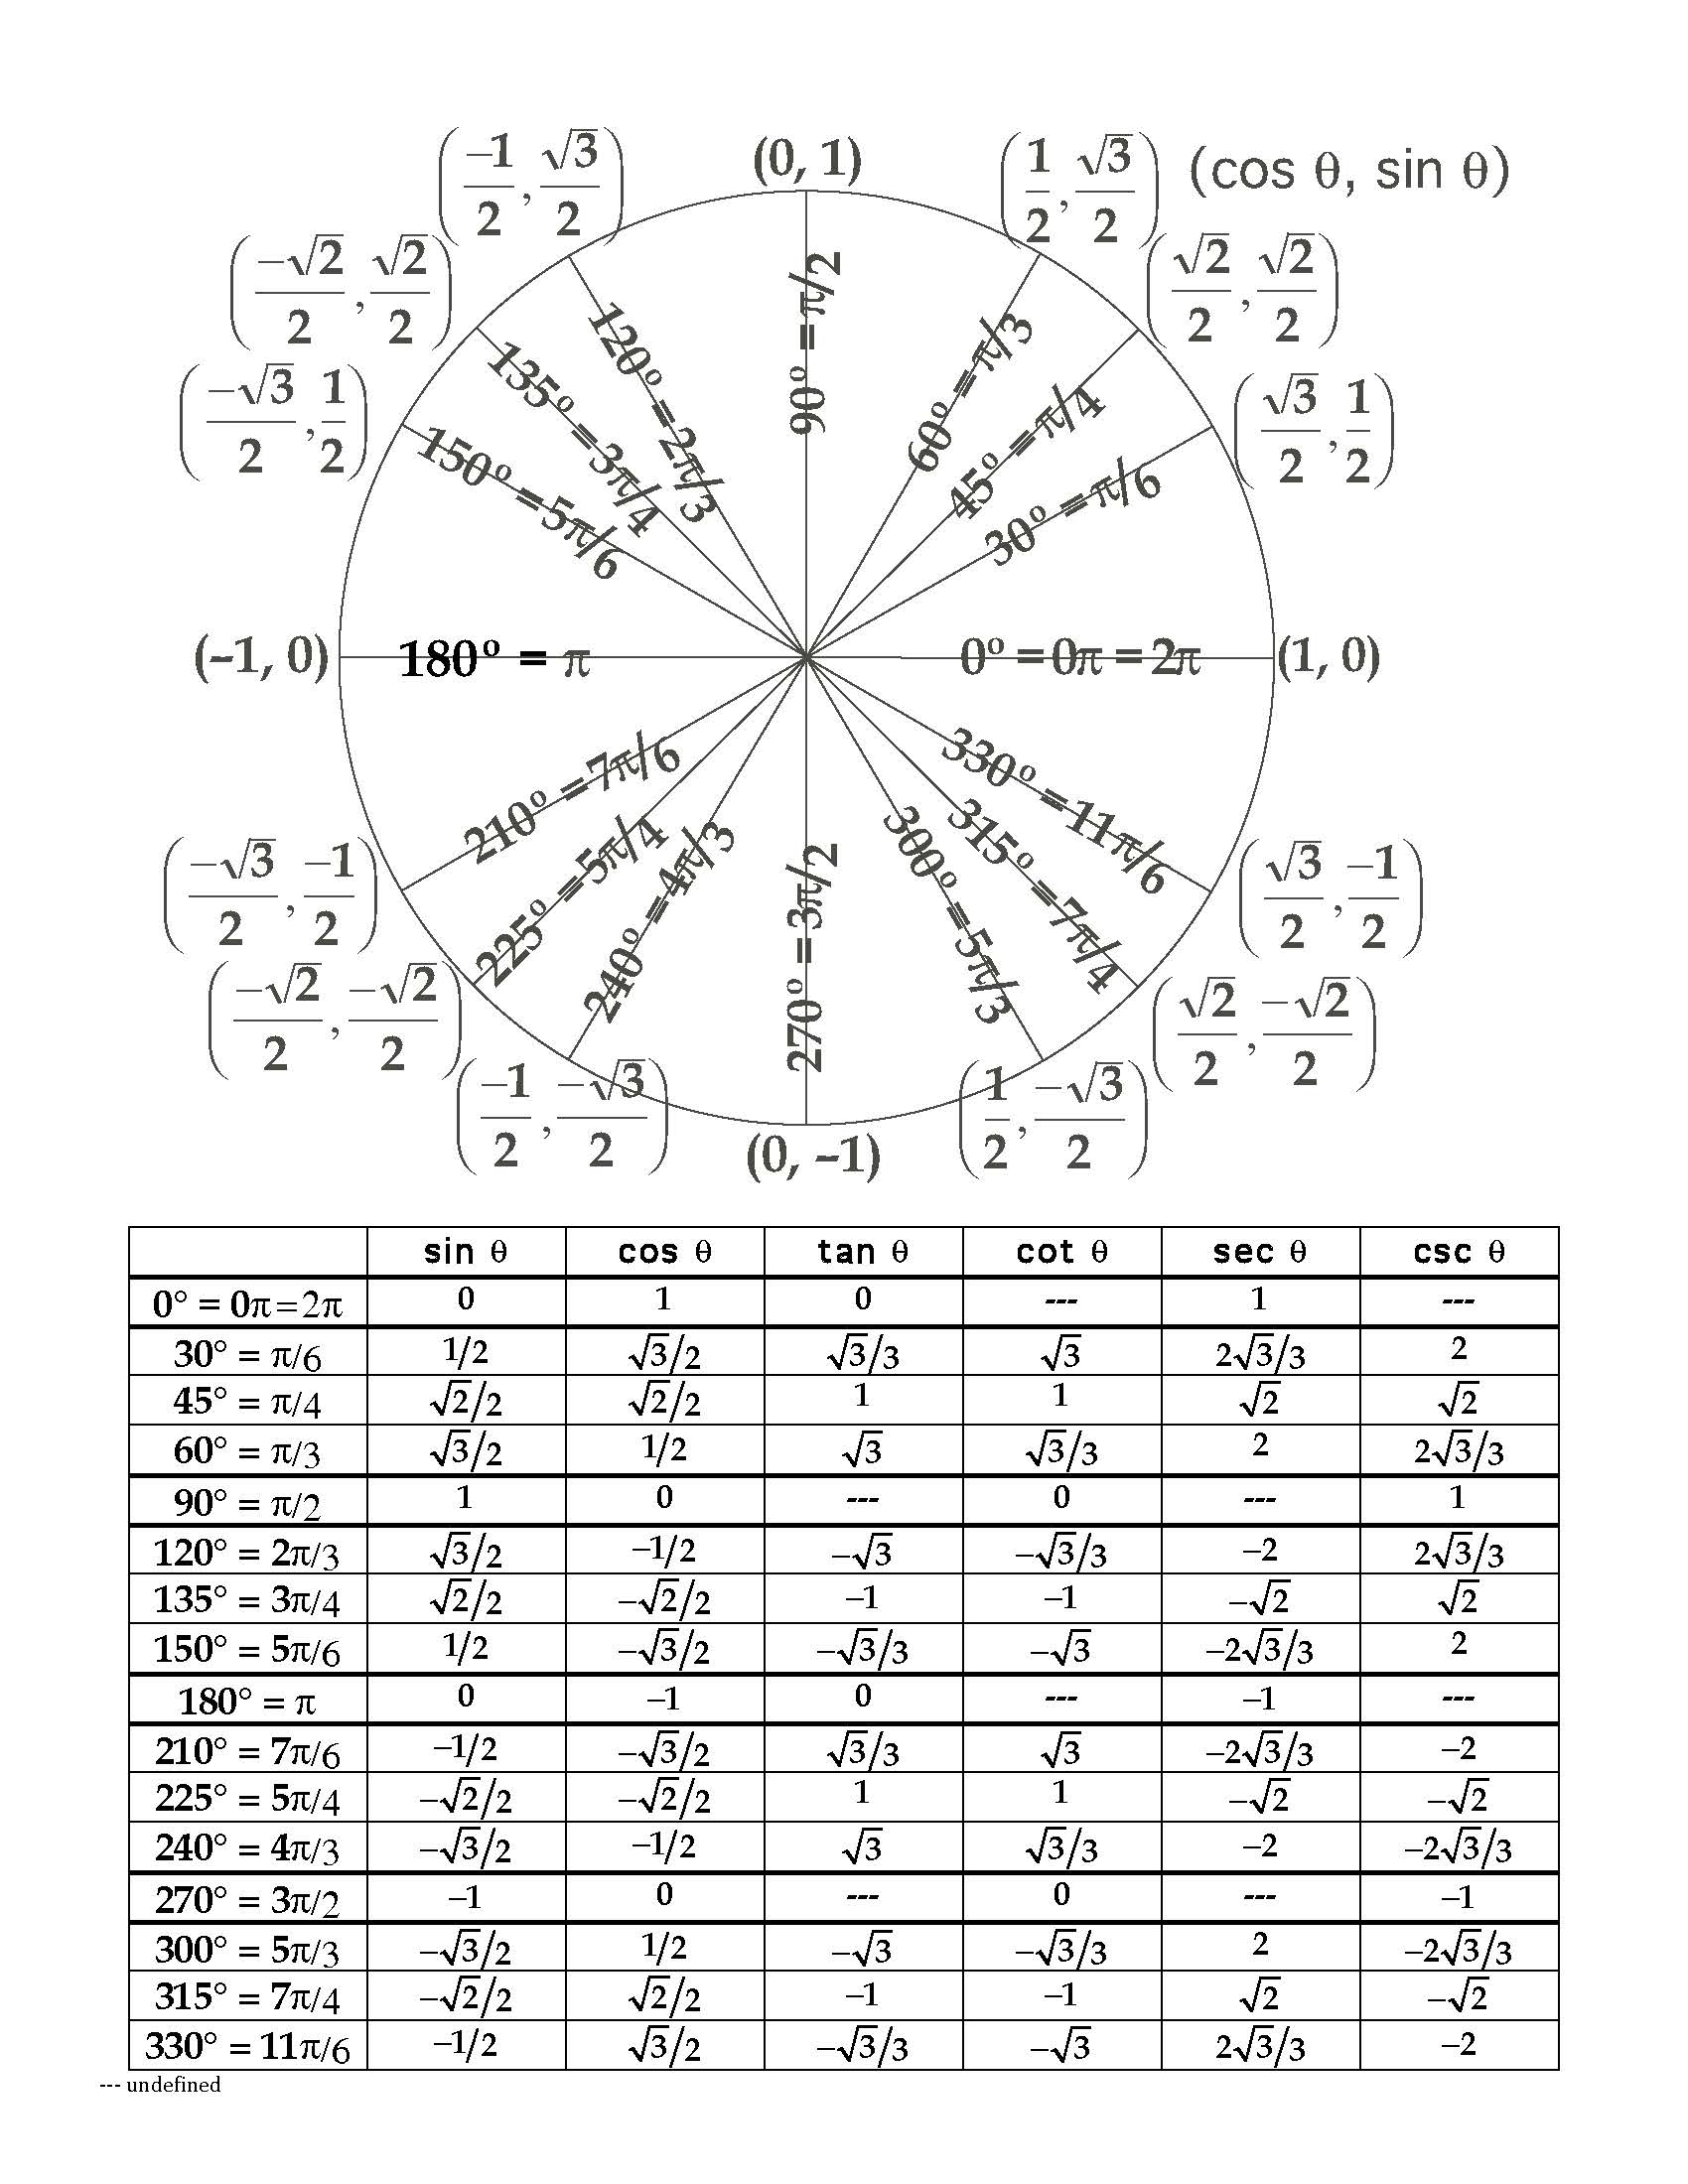
\includegraphics[width=3.5in]{UnitCircleChart.jpg}
    \label{fig:UnitCircleCht}
    \caption{The Unit Circle}
  \end{center}
\end{figure}

\section{Trigonometric Identities}
\subsection{Reciprocal Identities}

\parbox{1.5in}{\begin{eqnarray*}
\sin\theta &=& \frac{1}{\csc\theta} \\
\cos\theta &=& \frac{1}{\sec\theta} \\
\tan\theta &=& \frac{1}{\cot\theta}
\end{eqnarray*}}
\hfill
\parbox{1.5in}{\begin{eqnarray*}
\csc\theta &=& \frac{1}{\sin\theta} \\
\sec\theta &=& \frac{1}{\cos\theta} \\
\cot\theta &=& \frac{1}{\tan\theta}
\end{eqnarray*}}

\subsection{Quotient Identities}
\begin{eqnarray*}
\tan\theta &=& \frac{\sin\theta}{\cos\theta} \\
\cot\theta &=& \frac{\cos\theta}{\sin\theta}
\end{eqnarray*}

\subsection{Pythagorean Identities}
\begin{eqnarray*}
\sin^{2}\theta + \cos^{2}\theta &=& 1 \\
1 + \tan^{2}\theta &=& \sec^{2}\theta \\
1 + \cot^{2}\theta &=& \csc^{2}\theta
\end{eqnarray*}

\end{document}
